\documentclass[../ThesisDoc]{subfiles}
\begin{document}

\providecommand{\rootdir}{..}

The external context asks counterparts an \emph{opinion} about a candidate.
An \textbf{opinion} is the \emph{inner coherence} of the agent being asked.
% This context plays crucial role in coherence property \ref{eq:coh-fun-independ}.
It combines the internal coherences of the agent itself and other agents,
mentioned in the assessed candidate.

% To speedup opinions assessment, the agents should share the newly created classes.
% Any class $c_i \sim \left< \dots, g_i, p_i, r_i, \dots \right>$, created by
% any agent of triple $\left< g_i, p_i, r_i \right>$, should be sent by that
% agent to the rest of the triple. A received class must be added to agent's
% classes pool.

% \begin{figure}[h]
%   \label{fig:CandidatesShareOpinions}
%   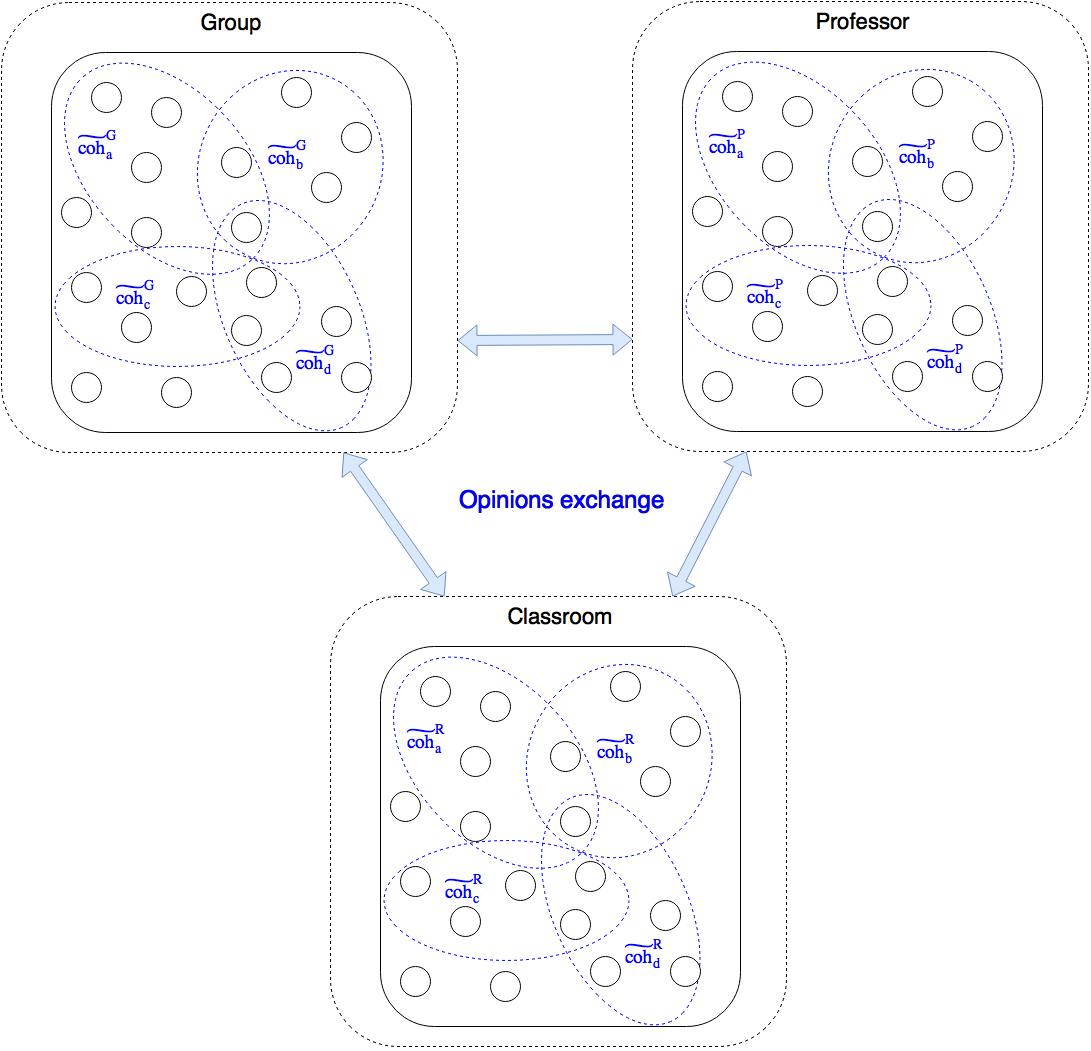
\includegraphics[width=\textwidth]{\rootdir/img/CandidatesShareOpinions.png}
%   \caption{Agents exchange thier \emph{internal coherences} of the candidates
%             $\cohi^a_i = \cohi[a](c_i)$ in form \emph{opinions}.
%           }
% \end{figure}

The internal coherences are combined using \emph{common goal} function $\Gamma$.
The common goal must combine coherence values, making no difference
between value origins.

The simplest \emph{common goal} functions are \emph{product} $\prod$
and \emph{mean} $\frac{\sum_n}{n}$.


% \red{The $\Gamma$ function ensures \ref{eq:coh-fun-independ} coherence property,
% that permits to avoid \dots}


\end{document}
